\documentclass[sigplan,screen]{format/acmart}
\usepackage{todonotes}
\usepackage{graphicx}
\usepackage{wrapfig}

\newcommand{\TODO}[1]{\todo[inline]{#1}}

%\setcopyright{acmcopyright}
\setcopyright{Apachee 2.0}
\copyrightyear{2022}
\acmYear{2022}
\acmDOI{XXXXXXX.XXXXXXX}

\acmConference[University of Virginia Data Science Capstone 2022]{MLCommons Earthquake Science Benchmark}{Jan. 22 -- Aug. ??,
  2022}{Charlotsville, VA}
\acmBooktitle{Woodstock '18: ACM Symposium on Neural Gaze Detection,
  June 03--05, 2018, Woodstock, NY} 
\acmPrice{0.00}
\acmISBN{TBD}
%%\acmSubmissionID{123-A56-BU3}
%%\citestyle{acmauthoryear}

\begin{document}

\title{MLCommons Earthquake Science Benchmark}

\author{Thomas Butler}
\email{trovato@corporation.com}
\author{G.K.M. Tobin}
\email{webmaster@marysville-ohio.com}
\affiliation{%
  \institution{University of Virginia}
  \city{Charlotsville, VA}
  \country{USA}}

\author{Robert Knuuti}
\orcid{0000-0003-2614-0899}
\affiliation{%
  \institution{University of Virginia}
  \city{Charoletteville}
  \country{USA}}
\email{robert.knuuti@gmail.com}

\author{Jake Kolessar}
\affiliation{%
  \institution{University of Virginia}
  \city{Charlottesville}
  \state{VA}
  \postcode{22911}
  \country{United States}}
\email{jakekolessar@gmail.com}

\author{Geoffrey C. Fox}
\affiliation{%
  \institution{University of Virginia}
  \streetaddress{Biocomplexity Institute
Town Center Four
994 Research Park Boulevard}
  \city{Charlottesville}    
  \state{VA}
  \postcode{22911}
  \country{USA}}
\email{gcfexchange@gmail.com}

\author{Gregor von Laszewski}
\orcid{0000-0001-9558-179X}
\affiliation{%
  \institution{University of Virginia}
  \streetaddress{Biocomplexity Institute
Town Center Four
994 Research Park Boulevard}
  \city{Charlottesville}    
  \state{VA}
  \postcode{22911}
  \country{USA}}
\email{laszewski@gmail.com}

\author{Judy Fox}
\affiliation{%
  \institution{University of Virginia}
  \city{Charlottesville}      
  \state{VA}
  \postcode{22911}
  \country{USA}}
\email{cwk9mp@virginia.edu}

\renewcommand{\shortauthors}{Buttler, Knuuti, Kolesar, Fox, von Laszewski}

\begin{abstract}
TBD
\end{abstract}

%% see http://dl.acm.org/ccs.cfm.
\begin{CCSXML}
<ccs2012>
 <concept>
  <concept_id>10010520.10010553.10010562</concept_id>
  <concept_desc>Computer systems organization~Embedded systems</concept_desc>
  <concept_significance>500</concept_significance>
 </concept>
 <concept>
  <concept_id>10010520.10010575.10010755</concept_id>
  <concept_desc>Computer systems organization~Redundancy</concept_desc>
  <concept_significance>300</concept_significance>
 </concept>
 <concept>
  <concept_id>10010520.10010553.10010554</concept_id>
  <concept_desc>Computer systems organization~Robotics</concept_desc>
  <concept_significance>100</concept_significance>
 </concept>
 <concept>
  <concept_id>10003033.10003083.10003095</concept_id>
  <concept_desc>Networks~Network reliability</concept_desc>
  <concept_significance>100</concept_significance>
 </concept>
</ccs2012>
\end{CCSXML}

\ccsdesc[500]{Computer systems organization~Embedded systems}
\ccsdesc[300]{Computer systems organization~Redundancy}
\ccsdesc{Computer systems organization~Robotics}
\ccsdesc[100]{Networks~Network reliability}

%%
%% Keywords. The author(s) should pick words that accurately describe
%% the work being presented. Separate the keywords with commas.
\keywords{MLCommons, Science AI Benchmark, Earthquake, Deep Learning}

\maketitle

\section{Introduction}

Several research efforts have been executed over the years to establish a set of leading factors that could be used to predict where an earthquake could occur.
Not only is this an algorithmically complex problem, but it is also computationally difficult to perform\cite{fox2022aiforscience}.
The intersection of these two elements create an ideal environment for building benchmarks.
By establishing a rigorous process to build a repeatable models, we can establish a benchmark to not only measure the performance of high performance supercomputers, but also take steps to building a stronger understanding of what models perform best to predict when and earthquake could occur.

For this study, we review the following models across various hardware platforms to establish this benchmark:
\begin{itemize}
    \item pure (vanilla) recurrent neuronetwork
    \item spacio-temporal science transformer
    \item temporal fusion transformer
\end{itemize}

\subsection{MLCommons}

MLCommons is an open engineering organization that seeks to unify the engineering and machine learning communities through system benchmarks, open data, and best practices\ref{www-mlcommons}.
By using open data, a reference implementation for benchmarking, and executing best practices, you can build the necessary rigor to construct repeatable research to establish a basis when performing future analysis.

This organization will establish the dimensions for what is the minimally viable solution and to establish our comparison criteria across our models and the executions on the different hardware sets.

\TODO{Need to confirm what the criteria of the benchmark submission is.}


\subsection{Earthquake prediction}



Things to do: 

\begin{itemize}
    %% \item add presentation as cite,
    \item Review IEEE Presentation \cite{fox2022aiforscience}
    \item Review MLCommons \cite{www-mlcommons} 
    \item Use jabref \cite{www-jabrefg-org} for citation management
    \item Review Fox paper \cite{fox2021earthquake}
    \item Frequently check github \cite{www-mlcommons-eathquake}
    \item Read up on TFT \cite{www-onnen2021}
    \item Become familiar with the Attention Paper \cite{vaswani2017attention}
    \item Learn how to selfdeploy jupyterlab \cite{www-jupyterlab}
    \TODO{Is this the same as jupytext?}
        
    \item Begin to learn about papermill \cite{www-papermill} \TODO{Rivanna's core configurations might be a bit limited on this front.  They do provide multiple versions of software (such as py2.7 and py3.8), but we may need to get permission to do something in userspace if we need to be very specific on a version of python.  Do we want to look into using tox, conda, or leave this up to the container ecosystem to solve?}
    \TODO{Gregor: add how to use conda and modules to switch python versions}
    \item virtualenv on rivanna for a particular python version.
    \item depends on Tensorflow
    \TODO{Below this line are objectives or targets to take the current modeling solution and mature it for other platforms / ecosystems.  Rivanna uses Lua's lmod ecosystem for jailing a process, and anaconda uses solved environments for dependencies that extend beyond just python modules.}
    \item Familiarize yourself with Rivanna's modules \cite{www-modules}  and conda \cite{www-conda} environments.
    \item pytorch \cite{www-pytorch}
    \TODO{There is interest in comparing pytorch and tensoflow}
    \item horovod \cite{www-horovod}
    \TODO{MLCommons project that can target a few platforms using a YAML contract.  Once we solve the target environment, we can likely target porting this way.}
    \TODO{Also, good news is Rivanna has a Singularity module  as an lmod (3.7.1), so we might be able to use that as a targeted runner without having to setup too much additional scaffolding.
    And if things work right, we could use the k8s module to do local deployments if we wanted to test out alternate execution paths. }
    \item mlcube \cite{www-mlcube} 
\end{itemize}

%\begin{figure}[h]
%  \centering
%  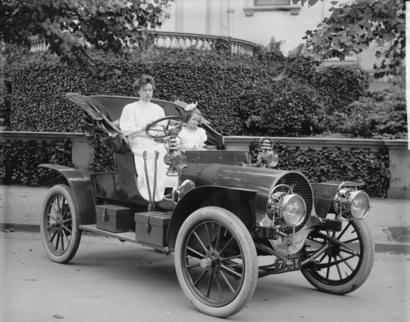
\includegraphics[width=\linewidth]{sample-franklin}
%  \caption{1907 Franklin Model D roadster. Photograph by Harris \&
%    Ewing, Inc. [Public domain], via Wikimedia
%    Commons. (\url{https://goo.gl/VLCRBB}).}
%  \Description{A woman and a girl in white dresses sit in an open car.}
% \end{figure}

\section{Benchmarks}

\subsection{Hardware}

\subsection{University of Virginia Rivanna}
\label{id:uva} 

UVA, Rivanna, A100, RTX3090, others may not have enough memory. 
\cite{www-rivanna}
\TODO{description of Rivanna on web page is not accurate.}

\subsection{Pearl}
\label{id:ral} 

Rutherford Appleton Laboratory (RAL), UK 
Pearl \cite{www-pearl-1}

\subsection{Summit}
\label{id:ornl} 

Oak Ridge National Labratory (ORNL), Summit \cite{www-summit}

\subsection{Perlmutter}
\label{id:nersc} 

National Energy Research Scientific Computing Center (NERSC), ...
\cite{www-perlmutter}

\subsection{Aurora}
\label{id:anl} 

Argonne National Laboratory (ANL), ... \cite{www-aurora}

\subsection{SDSC}
\label{id:sdcs} 

San Diego Super Computing Center, ... \cite(www-expanse}


\subsection {Nvidia DGX Workstation}

\label{id:dgx} DGX Fox \cite{www-dgx-station-a100}

\begin{table*}[htb]
    \caption{Overview of compute resources.}
    \label{tab:my_label}
    \centering
    \begin{tabular}{|r|l|l|r|l|l|}
        \hline
        Section & Organization & Machine  & Processors & GPUs &  Commissioned \\ 
        \hline
        \hline
         \ref{id:anl}   & ANL       &  Aurora \cite{www-aurora}         &            &      &    ??? 2022       \\
         \ref{id:ornl}  & ORNL      &  Summit \cite{www-summit}  &  27000  & NVIDIA Volta GPUs    &            \\
         \ref{id:nersc} & NERSC     &  Perlmutter \cite{www-perlmutter}         &    6000    & NVIDIA A100 & Jan 2022        \\
         \ref{id:sdsc}  & SDSC      &  Expanse \cite{www-expanse}         & 200&     NVIDIA V100 SMX2     &            \\
         \ref{id:uva}   & UVA       & Rivanna \cite{www-rivanna}  &      8       & NVIDIA A100 80GB     & Feb 2022 \\
         \ref{id:ral}   & RAL       &  Pearl \cite{www-pearl-1}        &   16         &  NVIDIA V100   &            \\
         \ref{id:dgx}   & Fox & DGX Staion A100 \cite{www-dgx-station-a100}  & 4 &  NVIDIA A100 80GB  & May 2021\\
         \hline
    \end{tabular}
\end{table*}


\begin{acks}
\TODO{Geoffrey: please add acknowledgement for funding, other acks}
\end{acks}

\bibliographystyle{ACM-Reference-Format}
\bibliography{paper-capstone-earthquake}

\section*{Biographies}

\TODO{wrapfigure does somehow not work in this template}

{\bf Thomas Butler}
\TODO{Thomas: fill out. See Gregor's example}

{\bf Robert Knuuti}
is a Graduate Student at University of Virginia's School of Data Science. He has over 10 years experience in system architecture and software engineering, and specializes in Development Operations and Cloud Computing. \TODO{Not sure what to add about research organizations; I'm generally not affiliated.}  He has constructed air gapped Continuous Integration and Continuous Delivery systems for multiple organizations each supporting more than 100 developers and has facilitated the construction of repeatable, tractable builds for users of these systems.

{\bf Jake Kolessar}
\TODO{Jake: fill out. See Gregor's example}

{\bf Geoffrey C. Fox}
\TODO{Geoffery: fill out}


%\begin{wrapfigure}{r}{0.25\columnwidth}
%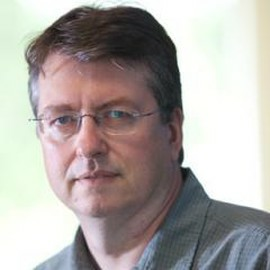
\includegraphics[width=0.24\columnwidth]{images/bio/gregor.png}
%\end{wrapfigure}

{\bf Gregor von Laszewski}
is a Research Professor at University of Virginia. He has more than 30 years of experience in parallel and distributed computing. Selected research organizations he worked in include NASA, Argonne National Laboratory, Indiana University. He is proud to have been contributing members of researchteams that invented hybrid parallel genetic algorithms, Grid computing, and the first large scale academic hybrid cloud, as well as the larges scientific bibliometric analysis of XSEDE in the world.




\appendix

\section{Manuals Developed}

The following manuals have been developed by the team:

\begin{itemize}
    \item Introduction to Python \cite{las-intro-python}
\end{itemize}

\clearpage 

\section{Todo}

\listoftodos

Robert: I am moving the rough notes into our github repo and made a 

\begin{itemize}
\item \href{https://github.com/cybertraining-dsc/capstone-eartquake/blob/main/TODO.md}{TODO.md} 
\end{itemize}

file that we can use to build a simple list of things we want to do.  I'll leave them in the overleaf for now, but I feel like that's not a good home for that type of information given that it's mean to be the paper to submit on the subject.

\TODO{Not sure if we want to talk about building tasks / kanban boards to track the different parts of work we'll be doing each week.  Additionally, it might be good to decide on some core roles to make sure things don't fall through the cracks (roles like recorder, scheduler, reviewer, et al...); the non-technical stuff for now, and then we can get into the more specific things once we pass the initial knowledge rampup}
\TODO{We now have a project board for this semester, milestones, and issues.}

\end{document}
\endinput
%%
%% End of file `sample-sigplan.tex'.
